\problemname{Anti-Tetris}

\illustration{0.21}{non-perfect-tetris.png}{
    The perfect example of a non-perfect \emph{Tetris} grid.
    CC BY-NC 2.0 by Richard Buitron on \href{https://www.flickr.com/photos/35973370@N03/3352142819}{Flickr}
}

\newcommand{\maxhwIn}{100}
\newcommand{\maxhwOut}{1000}

In the game \emph{Tetris},
the goal is to position blocks falling down a grid as well as possible.
\emph{Before} the block falls down, the player can shift the block to the left and
right, and rotate it in steps of $90$ degrees.
Then, the block falls down vertically until it hits another block.
Completely filling a row removes this row from the grid, clearing up space for more falling blocks.

You have played this game one too many times, and to shake things up, you decide to play \emph{Anti-Tetris}:
instead of controlling the positioning of the blocks falling down,
the goal is to design a Tetris grid that will perfectly fit a given block. That
is, a grid such that after optimally positioning the new block, all rows of the grid
are cleared and no filled cells remain.

As an example, consider the first sample case, shown in Figure~\ref{fig:tetris}.
The input block can be rotated clockwise $90$ degrees and shifted left to
make it fit exactly and clear all rows of the grid once it touches down.

\begin{figure}[h]
    \centering
    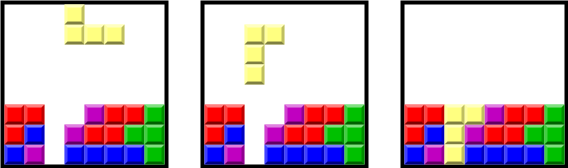
\includegraphics[width=0.9\textwidth]{tetris-sample-1.drawio.pdf}
    \caption{
        Visualization of the first sample case.
        The falling block (the input, light yellow) perfectly fits in the Tetris grid (the output, other colours).
    }
    \label{fig:tetris}
\end{figure}

\begin{Input}
    The input consists of:
    \begin{itemize}
        \item One line with two integers $h$ and $w$ ($1\leq h,
    w\leq \maxhwIn$), the height and width of the Tetris block that is about to
    enter the grid.
        \item $h$ lines with $w$ characters, each character being either `\texttt{\#}' or `\texttt{.}',
            representing a filled or unfilled cell of the block, respectively.
    \end{itemize}
    The input block is a single orthogonally\footnotemark{} connected component and exactly fits in the
    $w \times h$ bounding box,~i.e.~the first and last row and column contain at
    least one `\texttt{\#}'.
    \footnotetext{
        Two cells are orthogonal neighbours if and only if they are horizontal or vertical neighbours.
    }
\end{Input}

\begin{Output}
    If there exists no Tetris grid that perfectly fits the input block, output ``\texttt{impossible}''.
    Else, output a grid such that placing the the input block optimally removes all rows, in the following format:

    \begin{itemize}
        \item Two integers $h, w$ ($1\leq h, w\leq \maxhwOut$), the height and width of the Tetris grid.
        \item $h$ strings with $w$ characters, each character being either `\texttt{\#}' or `\texttt{.}',
            representing a filled or unfilled cell in the Tetris grid, respectively.
    \end{itemize}

    A row in the output grid may not be completely filled before the block is added,
    since such a row would already have been removed by the game.

    Note that it is not required to print empty rows at the top of the output grid,
    since the block can be rotated and shifted to the left and right \emph{before} it falls down.

    If there are multiple valid solutions, you may output any one of them.
\end{Output}
